The aim of this coursework is to implement and train a fully connected neural net to classifiy emotions using images of faces.
There are 7 emotions, namely: anger, disgust, fear, happiness, sadness, surprise and neutral.
This report discusses our approach and findings.
First, we discuss the theory behind neural nets.
Next, we explain how we tuned our neural net's hyperparameters
and provide an analysis of our model using metrics such as confusion matrices or recall rates.
We conclude with an exploration of neural net state of the art explorat

But first, what is neural network?
Neural networks aim to mimic the biological neural network present in the human brain.
Let us begin by explaining the concept of a neuron.

\begin{figure}[!ht]
    \centering
    \subfloat[neuron]{{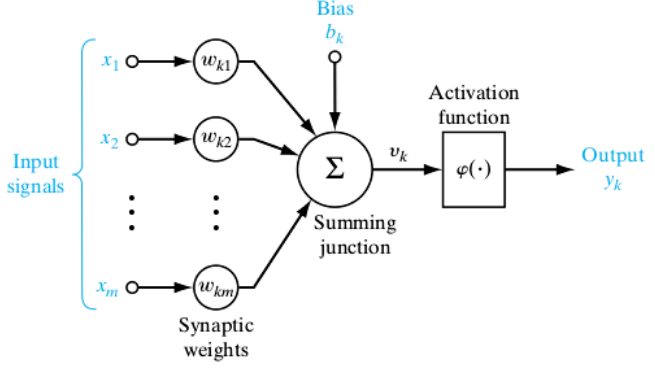
\includegraphics[scale = 0.35]{src/diagrams/neuron_diagram.png}}}
    \qquad
    \subfloat[neural net architecture]{{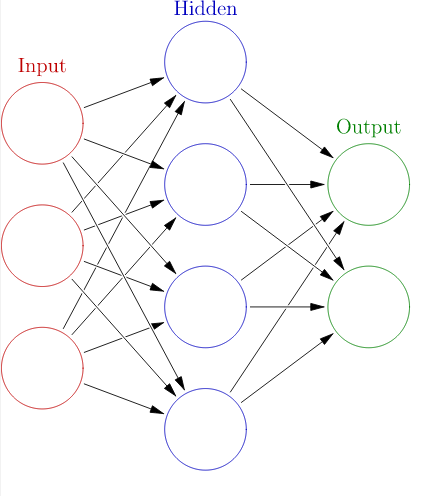
\includegraphics[scale = 0.35]{src/diagrams/neural_net_diagram.png}}}   
\end{figure}

A neuron takes in several inputs and produces a single output, as represented in the picture above.
A neuron sums all inputs weighted by their respective weights,
adds a bias and then inputs this into an activation function to produce a single output.

A neural network is is composed of layers of neurons,
such that each neuron's output is an input to all of the next layer's neurons.
The neural net architecture diagram above, shows three different types of layers.
An input layer contains a neuron for each data input's elements, which simply outputs the element it is given.
A hidden layer's neuron has a weight for each of the inputs connected to them,
and produces a single output as described earlier.
An output layer has an neuron for each output you wish to train your net to predict.
In this coursework, when we train a net to predict the emotion of a given image,
the net's output layer will have 7 neurons, one for each emotion.
Now that we have the basics down, let us now explore how a neural net works.

